\subsubsection{generation.tunnelgeneration}
    \textit{Tunnelgeneration} ist dafür verantwortlich einen Tunnel zu generieren, der andere Segmente einer Karte, 
    wie einen Ruam oder eine Kuppel, mit einander verbindet. Die Tunnel (\textit{ITunnel}) werden prozedural generiert 
    und sind von einem Seed abhängig.\par

    \begin{figure}[htbp]
        \centering
        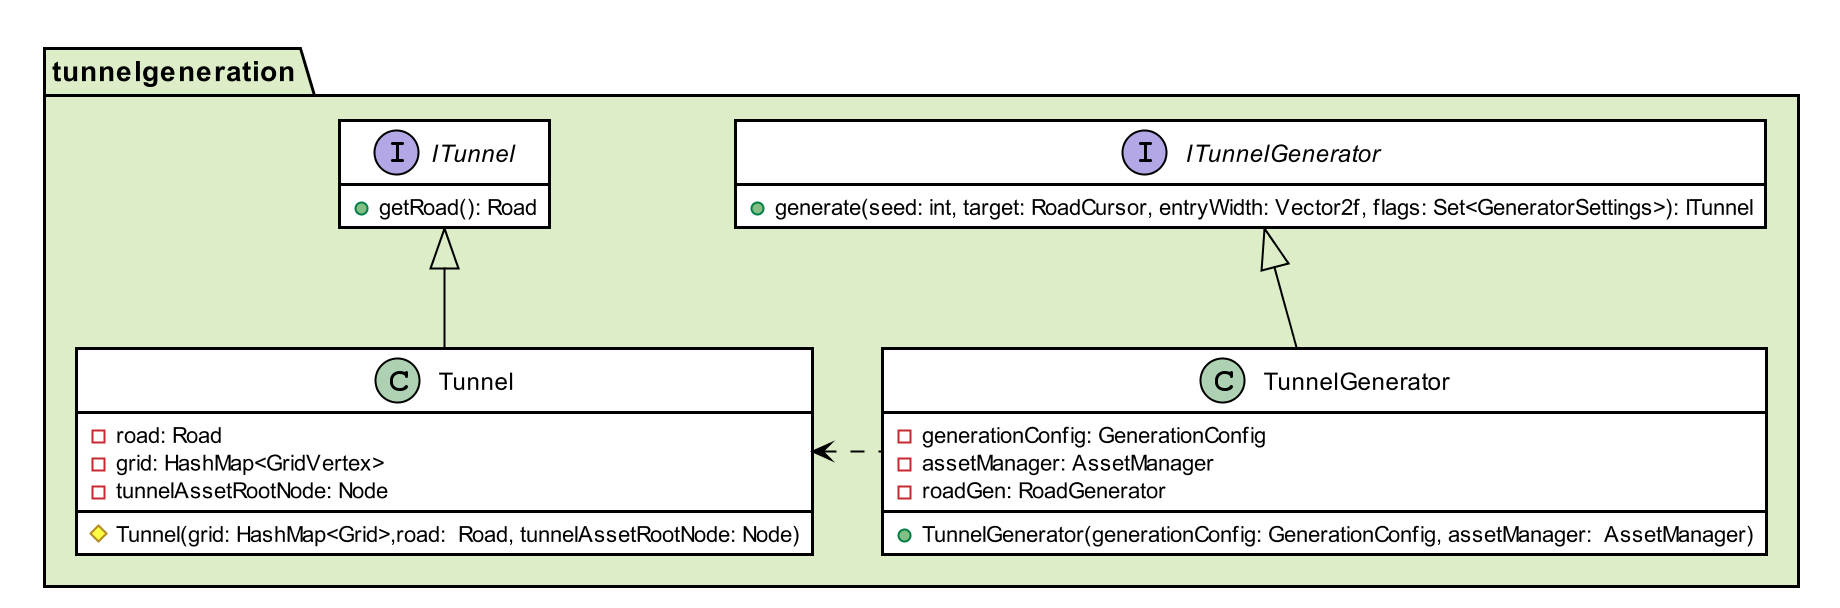
\includegraphics[width=\linewidth]{./Generierung/Bilder/tunnelgeneration.png}
        \caption{Klassendiagramm tunnelgeneration}
    \end{figure}


        \paragraph{\underline{ITunnelGenerator}} \mbox{}\par
            Schnittstelle um die Generierung eines Tunnels zwischen 2 Punkten anzuregen.\par
            
            \textbf{Methoden}					
            \begin{itemize}
                \item  \textit{+ generate(int seed, RoadCursor target, Vector2f entryWidth, Set<GeneratorSettings> flags): ITunnel}
                    \begin{leftbar}[0.9\linewidth]
                        Generiert einen Tunnel zwischen 2 Punkten, abhängig vom Seed und ggf. von flags.\\
                        \textbf{@param seed} Zum bestimmen von Pseuozufallswerten, die die Generierung bestimmen.\\
                        \textbf{@param target} Zielpunkt des zu generierenden Tunnels.\\
                        \textbf{@param entryWidth} Dimensionen für den Eingang des Tunnels.\\
                        \textbf{@param flags} Menge an Parametern, die als Präferenzen zur Generierung dienen.\\
                        \textbf{@return} Datenstruktur (\textit{ITunnel}), die einen Tunnel beschreibt.
                    \end{leftbar}   
            \end{itemize}
    
    
        \pagebreak
        \paragraph{\underline{TunnelGenerator}} \mbox{}\par
            Konkrete Imlementierung von \textit{ITunnelGenerator}, implementiert die Konkrete Generierungsfunktion für einen Tunnel
            zwischen 2 Punkten.\par
            
            \textbf{Attribute}
            \begin{itemize}
                \item  \textit{- GenerationConfig generationConfig} 
                    \begin{leftbar}[0.9\linewidth]
                        Datenstruktur, die Parameter für die Generierung hält.
                    \end{leftbar}
                
                \item  \textit{- AssetManager assetManager} 
                    \begin{leftbar}[0.9\linewidth]
                        Von \textit{JMonkey} vordefinierte Klasse, zum verwalten von Assets.
                    \end{leftbar}
                
                \item  \textit{- IRoadGenerator roadGen} 
                    \begin{leftbar}[0.9\linewidth]
                        Ist für die Generierung eines Streckenverlaufs verantwortlich.
                    \end{leftbar}
            \end{itemize}

            \textbf{Methoden}					
            \begin{itemize}
                \item  \textit{+ TunnelGenerator(GenerationConfig generationConfig, AssetManager assetManager)}
                    \begin{leftbar}[0.9\linewidth]
                        Konsrtuktor für \textit{TunnelGenerator}.\\
                        \textbf{@param generationConfig} Datenstruktur, die Parameter für die Generierung hält.\\
                        \textbf{@param assetManager}  Von \textit{JMonkey} vordefinierte Klasse, zum verwalten von Assets.
                    \end{leftbar} 
            \end{itemize}
    
    
       
        \paragraph{\underline{ITunnel}} \mbox{}\par
           Schnittstelle einer Datenstruktur, die einen Tunnel zwischen 2 Punkten beschreibt.\par

            \textbf{Methoden}					
            \begin{itemize}
                \item  \textit{+ generateSceneGraph(): Node}
                    \begin{leftbar}[0.9\linewidth]
                        Berechnet Scenegraph des Tunnelabschnitts und gibt ihn zurück.\\
                        \textbf{@return}  Verwendet wie in \textit{JMonkey}, wird übergeben um den Tunnel in einer Szene darzustellen.
                    \end{leftbar}

                \item  \textit{+ getRoad(): Road}
                    \begin{leftbar}[0.9\linewidth]
                        Gibt die Straße (\textit{Road}), die durch den Raum verläuft, zurück.\\
                        \textbf{@return} Repräsentiert die Straße in dem Raum.
                    \end{leftbar}     
            \end{itemize}
        
        
        \pagebreak
        \paragraph{\underline{Tunnel}} \mbox{}\par
            implementiert \textit{ITunnel}, stellt eine konkrete Datensturktur für einen Tunnel dar.\par
            
            \textbf{Attribute}
            \begin{itemize}
                \item  \textit{- Road road} 
                    \begin{leftbar}[0.9\linewidth]
                        Datenstruktur die eine Straße, die durch den Raum verläuft, repräsentiert.
                    \end{leftbar}
                
                \item  \textit{- HashMap<GridVertex> grid} 
                    \begin{leftbar}[0.9\linewidth]
                        Das Gitter des Tunnels, das verschiedene Stati pro \textit{GridVertex} speichert.
                    \end{leftbar}
                
                \item  \textit{- Node tunnelAssetRootNode} 
                    \begin{leftbar}[0.9\linewidth]
                        Verwendet wie in \textit{JMonkey}, hier soll der Tunnel angehängt werden.
                    \end{leftbar}
            \end{itemize}

            \textbf{Methoden}					
            \begin{itemize}
                \item  \textit{\# Tunnel(HashMap<Integer,GridVertex> grid, Road road, Node tunnelAssetRootNode)}
                    \begin{leftbar}[0.9\linewidth]
                        Konsrtuktor für \textit{Tunnel}.\\
                        \textbf{@param gird} Das Gitter des Tunnels, das verschiedene Stati pro \textit{GridVertex} speichert.\\
                        \textbf{@param road} Repräsentiert die Straße, die durch den Tunnel verläuft.\\
                        \textbf{@param tunnelAssetRootNode} Verwendet wie in \textit{JMonkey}, hier soll der Tunnel angehängt werden.
                    \end{leftbar}   
            \end{itemize}



